\chapter{TINJAUAN PUSTAKA}

\section{Subbab Derajat Pertama}
Gunakan \texttt{$\backslash$citet\{\}} untuk melakukan kutipan dengan nama penulis disebutkan dalam kalimat. Contoh: \citet{knuth:1984} berpendapat bahwa .... 

Gunakan \texttt{$\backslash$citep\{\}} untuk melakukan kutipan dengan nama penulis tidak disebutkan dalam kalimat. Contoh: \LaTeX \, adalah ... \citep{latex:companion}. Perhatikan bahwa jika banyak penulis antara 3 sampai 5 orang, maka saat sitasi pertama kali semua penulis dituliskan. Namun, untuk selanjutnya akan ditulis 1 nama penulis pertama
dilanjutkan dengan "dkk" seperti ini \citep{latex:companion}.

\begin{equation}
    e^{i\pi}+1=0.
    \label{eq:euler}
\end{equation}
Persamaan \eqref{eq:euler} merupakan salah satu persamaan matematika terindah yang pernah saya lihat.

Vektor merupakan anggota ruang vektor. Definisi ruang vektor sebagai berikut.
\begin{definition}
    Himpunan tak-kosong $V$ disebut ruang vektor jika ....
    \label{def:ruangvektor}
\end{definition}
Berdasarkan Definisi \ref{def:ruangvektor}, kita dapat mengetahui bahwa suatu ....
Berikut ini adalah contoh ruang vektor riil.
\begin{example}
    Himpunan $C[0,1] = \{f:[0,1] \to \mathbb{R}\} | f \mbox{kontinu}$ merupakan ruang vektor.
\end{example}

Ruang vektor mempunyai sifat sebagai berikut.
\begin{theorem}
    Diberikan ruang vektor $V$ dan subruang $W$ dari $V$. Ruang vektor $V$ dapat ditulis sebagai
	\begin{equation}
		V = W \oplus W^{\perp}. \label{eq:dekomposisiruangvektor}
	\end{equation}
    \label{thm:gramschmidt}
\end{theorem}

\begin{proof}
    \lipsum[1]
\end{proof}

Berdasarkan Teorema \ref{thm:gramschmidt}, persamaan \eqref{eq:dekomposisiruangvektor} berguna dalam proses Gram-Schimdt.

\begin{lemma}
    Elemen nol pada grup $G$ bersifat tunggal.
\end{lemma}

\begin{corollary}
    Dekomposisi ruang vektor bersifat unik jika ...
\end{corollary}

\begin{remark}
    Lorem ipsum dolor sit amet, consectetuer adipiscing elit.
\end{remark}

\begin{figure}[H]
    \centering
    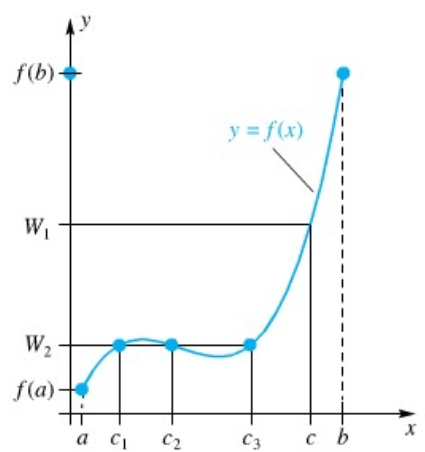
\includegraphics[width=0.5\linewidth]{gambar/teo_nilai_antara.png}
    \caption{Ilustrasi Teorema Nilai Antara}
    \caption*{\small \citep{varberg2007calculus}} % sumber gambar ditulis seperti ini jika gambar bukan buatan Anda sendiri
    \label{fig:teonilaiantara}
\end{figure}

Tambahkan ", telah diolah kembali" setelah sitasi sumber jika Anda sedikit menambahkan/memodifikasi gambar dari sumber yang Anda dapatkan. Misalkan gambar pada halaman selanjutnya sudah saya modifikasi.
\begin{figure}[H]
    \centering
    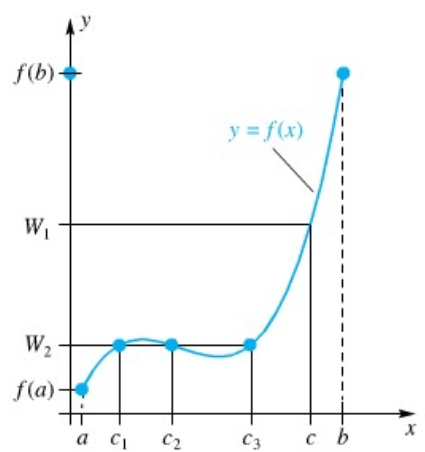
\includegraphics[width=0.5\linewidth]{gambar/teo_nilai_antara.png}
    \caption{Ilustrasi Teorema Nilai Antara 2}
    \caption*{\small \citep{varberg2007calculus}, telah diolah kembali} % sumber gambar ditulis seperti ini jika gambar bukan buatan Anda sendiri
    \label{fig:teonilaiantara2}
\end{figure}

Berikut adalah contoh tabel dalam \LaTeX.
\begin{table}[H]
    \centering
    \caption{Contoh Tabel 1}
    \begin{tabular}{|c|c|}
        \hline
        1 & 2 \\
        \hline
        3 & 4\\
        \hline
    \end{tabular}
    \label{tab:my_table}
\end{table}

\begin{table}[H]
    \centering
    \caption{Contoh Tabel 2}
    \begin{tabular}{ |c|c|c| } 
        \hline
        cell1 & cell2 & cell3 \\ 
        \hline
        cell4 & cell5 & cell6 \\ 
        cell7 & cell8 & cell9 \\ 
        \hline
    \end{tabular}
    \label{tab:my_label2}
\end{table}

\begin{remark}
    Ingat bahwa \textit{caption} serta sumber untuk gambar berada di bawah gambar, sedangkan untuk tabel berada di atas tabel.
\end{remark}
\subsection{Subbab Derajat Kedua}
\lipsum[1]

\subsubsection{Subbab Derajat Ketiga}
\lipsum[1]